% Figure from MATH 556 notes, section 21. Compile with the notes preamble.
\begin{tikzpicture}[scale=1.1, >=stealth]
    \begin{scope}
        \draw[gray] (0,0) circle (1.4);
        \node[gray] at (-1.0,1.3) {$X$};
        \foreach \n in {1,...,6} {\fill (1.2/\n,0.25/\n) circle (1.3pt);}
        \node[above] at (1.2,0.25) {$y_1$};
        \node[above] at (0.6,0.125) {$y_2$};
        \fill[blue!70!black] (0,0) circle (1.5pt) node[below, blue!70!black] {$0$};
        \node[below] at (0.5,-0.6) {$\|y_n\|_X = \tfrac1n \to 0$};
    \end{scope}
    \draw[->, thick] (1.8,0) -- (3.0,0) node[midway, above] {$T$};
    \begin{scope}[xshift=5cm]
        \draw[gray] (0,0) circle (1.6);
        \node[gray] at (-1.2,1.5) {$Y$};
        \draw[dashed, red!75!black] (0,0) circle (0.8);
        \node[red!75!black, font=\scriptsize] at (0,-0.38) {$\|y\|_Y \le 1$};
        \foreach \n/\a in {1/20,2/70,3/130,4/190,5/250,6/320} {\fill ({(0.95+0.08*\n)*cos(\a)},{(0.95+0.08*\n)*sin(\a)}) circle (1.3pt);}
        \fill[blue!70!black] (0,0) circle (1.5pt) node[above, blue!70!black] {$T0 = 0$};
        \node[below] at (0,-1.7) {$\|T y_n\|_Y > 1$};
    \end{scope}
\end{tikzpicture}
